% Options for packages loaded elsewhere
\PassOptionsToPackage{unicode}{hyperref}
\PassOptionsToPackage{hyphens}{url}
%
\documentclass[
]{article}
\usepackage{amsmath,amssymb}
\usepackage{iftex}
\ifPDFTeX
  \usepackage[T1]{fontenc}
  \usepackage[utf8]{inputenc}
  \usepackage{textcomp} % provide euro and other symbols
\else % if luatex or xetex
  \usepackage{unicode-math} % this also loads fontspec
  \defaultfontfeatures{Scale=MatchLowercase}
  \defaultfontfeatures[\rmfamily]{Ligatures=TeX,Scale=1}
\fi
\usepackage{lmodern}
\ifPDFTeX\else
  % xetex/luatex font selection
\fi
% Use upquote if available, for straight quotes in verbatim environments
\IfFileExists{upquote.sty}{\usepackage{upquote}}{}
\IfFileExists{microtype.sty}{% use microtype if available
  \usepackage[]{microtype}
  \UseMicrotypeSet[protrusion]{basicmath} % disable protrusion for tt fonts
}{}
\makeatletter
\@ifundefined{KOMAClassName}{% if non-KOMA class
  \IfFileExists{parskip.sty}{%
    \usepackage{parskip}
  }{% else
    \setlength{\parindent}{0pt}
    \setlength{\parskip}{6pt plus 2pt minus 1pt}}
}{% if KOMA class
  \KOMAoptions{parskip=half}}
\makeatother
\usepackage{xcolor}
\usepackage[margin=1in]{geometry}
\usepackage{color}
\usepackage{fancyvrb}
\newcommand{\VerbBar}{|}
\newcommand{\VERB}{\Verb[commandchars=\\\{\}]}
\DefineVerbatimEnvironment{Highlighting}{Verbatim}{commandchars=\\\{\}}
% Add ',fontsize=\small' for more characters per line
\usepackage{framed}
\definecolor{shadecolor}{RGB}{248,248,248}
\newenvironment{Shaded}{\begin{snugshade}}{\end{snugshade}}
\newcommand{\AlertTok}[1]{\textcolor[rgb]{0.94,0.16,0.16}{#1}}
\newcommand{\AnnotationTok}[1]{\textcolor[rgb]{0.56,0.35,0.01}{\textbf{\textit{#1}}}}
\newcommand{\AttributeTok}[1]{\textcolor[rgb]{0.13,0.29,0.53}{#1}}
\newcommand{\BaseNTok}[1]{\textcolor[rgb]{0.00,0.00,0.81}{#1}}
\newcommand{\BuiltInTok}[1]{#1}
\newcommand{\CharTok}[1]{\textcolor[rgb]{0.31,0.60,0.02}{#1}}
\newcommand{\CommentTok}[1]{\textcolor[rgb]{0.56,0.35,0.01}{\textit{#1}}}
\newcommand{\CommentVarTok}[1]{\textcolor[rgb]{0.56,0.35,0.01}{\textbf{\textit{#1}}}}
\newcommand{\ConstantTok}[1]{\textcolor[rgb]{0.56,0.35,0.01}{#1}}
\newcommand{\ControlFlowTok}[1]{\textcolor[rgb]{0.13,0.29,0.53}{\textbf{#1}}}
\newcommand{\DataTypeTok}[1]{\textcolor[rgb]{0.13,0.29,0.53}{#1}}
\newcommand{\DecValTok}[1]{\textcolor[rgb]{0.00,0.00,0.81}{#1}}
\newcommand{\DocumentationTok}[1]{\textcolor[rgb]{0.56,0.35,0.01}{\textbf{\textit{#1}}}}
\newcommand{\ErrorTok}[1]{\textcolor[rgb]{0.64,0.00,0.00}{\textbf{#1}}}
\newcommand{\ExtensionTok}[1]{#1}
\newcommand{\FloatTok}[1]{\textcolor[rgb]{0.00,0.00,0.81}{#1}}
\newcommand{\FunctionTok}[1]{\textcolor[rgb]{0.13,0.29,0.53}{\textbf{#1}}}
\newcommand{\ImportTok}[1]{#1}
\newcommand{\InformationTok}[1]{\textcolor[rgb]{0.56,0.35,0.01}{\textbf{\textit{#1}}}}
\newcommand{\KeywordTok}[1]{\textcolor[rgb]{0.13,0.29,0.53}{\textbf{#1}}}
\newcommand{\NormalTok}[1]{#1}
\newcommand{\OperatorTok}[1]{\textcolor[rgb]{0.81,0.36,0.00}{\textbf{#1}}}
\newcommand{\OtherTok}[1]{\textcolor[rgb]{0.56,0.35,0.01}{#1}}
\newcommand{\PreprocessorTok}[1]{\textcolor[rgb]{0.56,0.35,0.01}{\textit{#1}}}
\newcommand{\RegionMarkerTok}[1]{#1}
\newcommand{\SpecialCharTok}[1]{\textcolor[rgb]{0.81,0.36,0.00}{\textbf{#1}}}
\newcommand{\SpecialStringTok}[1]{\textcolor[rgb]{0.31,0.60,0.02}{#1}}
\newcommand{\StringTok}[1]{\textcolor[rgb]{0.31,0.60,0.02}{#1}}
\newcommand{\VariableTok}[1]{\textcolor[rgb]{0.00,0.00,0.00}{#1}}
\newcommand{\VerbatimStringTok}[1]{\textcolor[rgb]{0.31,0.60,0.02}{#1}}
\newcommand{\WarningTok}[1]{\textcolor[rgb]{0.56,0.35,0.01}{\textbf{\textit{#1}}}}
\usepackage{graphicx}
\makeatletter
\def\maxwidth{\ifdim\Gin@nat@width>\linewidth\linewidth\else\Gin@nat@width\fi}
\def\maxheight{\ifdim\Gin@nat@height>\textheight\textheight\else\Gin@nat@height\fi}
\makeatother
% Scale images if necessary, so that they will not overflow the page
% margins by default, and it is still possible to overwrite the defaults
% using explicit options in \includegraphics[width, height, ...]{}
\setkeys{Gin}{width=\maxwidth,height=\maxheight,keepaspectratio}
% Set default figure placement to htbp
\makeatletter
\def\fps@figure{htbp}
\makeatother
\setlength{\emergencystretch}{3em} % prevent overfull lines
\providecommand{\tightlist}{%
  \setlength{\itemsep}{0pt}\setlength{\parskip}{0pt}}
\setcounter{secnumdepth}{5}
\usepackage[spanish]{babel}
\usepackage{fontspec}
\ifLuaTeX
  \usepackage{selnolig}  % disable illegal ligatures
\fi
\IfFileExists{bookmark.sty}{\usepackage{bookmark}}{\usepackage{hyperref}}
\IfFileExists{xurl.sty}{\usepackage{xurl}}{} % add URL line breaks if available
\urlstyle{same}
\hypersetup{
  pdftitle={Tarea 2},
  pdfauthor={José Ignacio Rojas Zárate, C16911; Montserrat Beirute Abarca, C10997; Valeria Vásquez Venegas, C18373},
  hidelinks,
  pdfcreator={LaTeX via pandoc}}

\title{Tarea 2}
\usepackage{etoolbox}
\makeatletter
\providecommand{\subtitle}[1]{% add subtitle to \maketitle
  \apptocmd{\@title}{\par {\large #1 \par}}{}{}
}
\makeatother
\subtitle{Estadística Actuarial II}
\author{José Ignacio Rojas Zárate, C16911 \and Montserrat Beirute
Abarca, C10997 \and Valeria Vásquez Venegas, C18373}
\date{07 de febrero de 2024}

\begin{document}
\maketitle

{
\setcounter{tocdepth}{2}
\tableofcontents
}
\newpage

\hypertarget{ejercicio-1}{%
\section{Ejercicio 1}\label{ejercicio-1}}

\textbf{Usando un algoritmo de integración por Montecarlo estime ln(2)
con un error absoluto de 10−3}

Considere la siguiente integral:
\[ \int_{0}^{1} \frac{\ln(x + 1)}{2} + \frac{1}{2} \, dx \].

\emph{Solución:}

Empezamos separando la integral en dos partes. Para
\(\int \frac{\ln(x + 1)}{2} \, dx\): Realizamos la sustitución
\(u = x + 1\) y \(du = dx\). Note que si
\(x \rightarrow 0 \Rightarrow u \rightarrow 1\) y si
\(x \rightarrow 1 \Rightarrow u \rightarrow 2\). Esta primera integral
se convierte en: \(\frac{1}{2} \int_{1}^{2} \ln(u) \, du\)

Ahora, se aplica la regla de integración por partes, donde
\(m = \ln(u) \Rightarrow dm = \frac{1}{u} du\) y
\(dv = 1 \Rightarrow v = u\):

\[ \frac{1}{2} \left( u \ln(u) \Big|_{1}^2 - \int_{1}^{2} u \, \frac{1}{u} du\right) \]

Esto se simplifica a:
\(\frac{1}{2} \left(\ln(2) - 1 \right) = \frac{\ln(2)}{2} - \frac{1}{2}\).

La otra parte de la integral original,
\(\int_{0}^{1} \frac{1}{2} \, dx = \frac{1}{2}\):

Por lo tanto, la solución a la integral es
\(\frac{\ln(2)}{2} - \frac{1}{2} + \frac{1}{2} = \ln(2)\).

Ahora, procedemos a aplicar el algoritmo de Montecarlo:

\begin{Shaded}
\begin{Highlighting}[]
\FunctionTok{set.seed}\NormalTok{(}\DecValTok{147}\NormalTok{) }\CommentTok{\# definimos una semilla}
\NormalTok{n }\OtherTok{\textless{}{-}}\DecValTok{10}\SpecialCharTok{\^{}}\DecValTok{4} \CommentTok{\# tamaño de la muestra}
\NormalTok{U }\OtherTok{\textless{}{-}}\FunctionTok{runif}\NormalTok{(n) }\CommentTok{\# genera un vector con distribución uniforme}

\NormalTok{g }\OtherTok{\textless{}{-}}\FunctionTok{Vectorize}\NormalTok{(}\ControlFlowTok{function}\NormalTok{(x) (}\FunctionTok{log}\NormalTok{(x }\SpecialCharTok{+} \DecValTok{1}\NormalTok{)}\SpecialCharTok{/}\DecValTok{2}\NormalTok{) }\SpecialCharTok{+}\NormalTok{ (}\DecValTok{1}\SpecialCharTok{/}\DecValTok{2}\NormalTok{) ) }\CommentTok{\# construimos la función g }

\FunctionTok{curve}\NormalTok{(g,}\DecValTok{0}\NormalTok{,}\DecValTok{1}\NormalTok{,}\AttributeTok{col=}\StringTok{"lightblue4"}\NormalTok{,}\AttributeTok{lwd=}\DecValTok{1}\NormalTok{,}\AttributeTok{main=}\StringTok{"Gráfico de g(X)"}\NormalTok{)}
\FunctionTok{grid}\NormalTok{()  }
\end{Highlighting}
\end{Shaded}

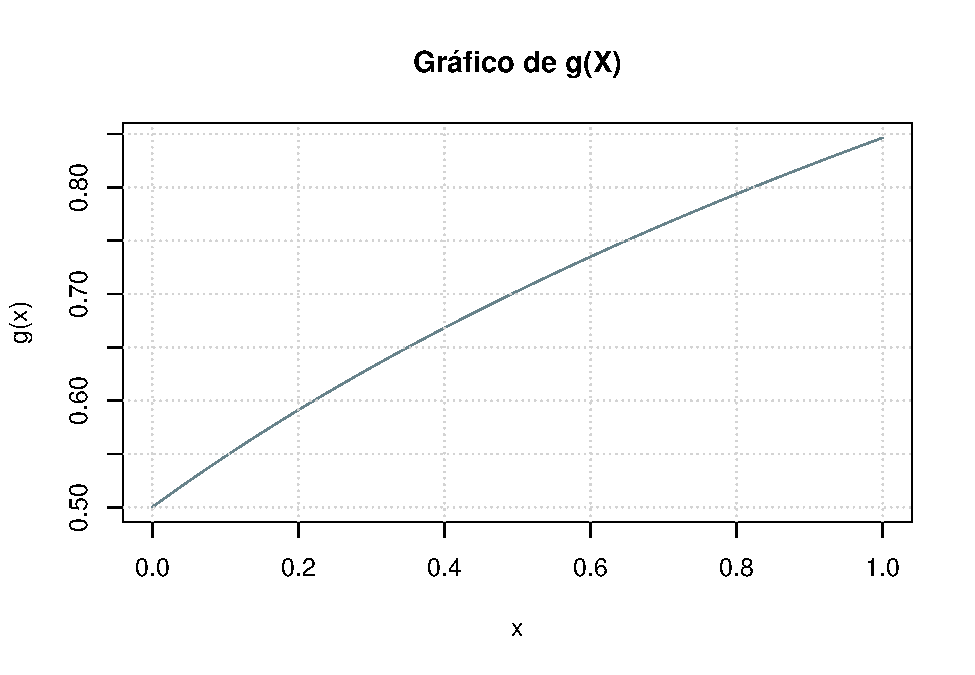
\includegraphics{tarea2_files/figure-latex/unnamed-chunk-1-1.pdf}

\begin{Shaded}
\begin{Highlighting}[]
\NormalTok{Y }\OtherTok{\textless{}{-}} \FunctionTok{g}\NormalTok{(U) }\CommentTok{\#genera el vector para cada observación}
\NormalTok{acumulado}\OtherTok{\textless{}{-}}\FunctionTok{cumsum}\NormalTok{(Y)}\SpecialCharTok{/}\NormalTok{(}\DecValTok{1}\SpecialCharTok{:}\NormalTok{n)}
\FunctionTok{plot}\NormalTok{(}\DecValTok{1}\SpecialCharTok{:}\NormalTok{n,acumulado,}\AttributeTok{col=}\StringTok{"lightblue4"}\NormalTok{,}\AttributeTok{type=}\StringTok{"l"}\NormalTok{,}\AttributeTok{ylab=}\StringTok{"Aproximación"}\NormalTok{,}\AttributeTok{xlab=}\StringTok{"Iteraciones"}\NormalTok{)}
\FunctionTok{abline}\NormalTok{(}\AttributeTok{h=}\FunctionTok{integrate}\NormalTok{(g,}\DecValTok{0}\NormalTok{,}\DecValTok{1}\NormalTok{)}\SpecialCharTok{$}\NormalTok{value,}\AttributeTok{col=}\StringTok{"coral2"}\NormalTok{,}\AttributeTok{lwd=}\DecValTok{1}\NormalTok{)}
\end{Highlighting}
\end{Shaded}

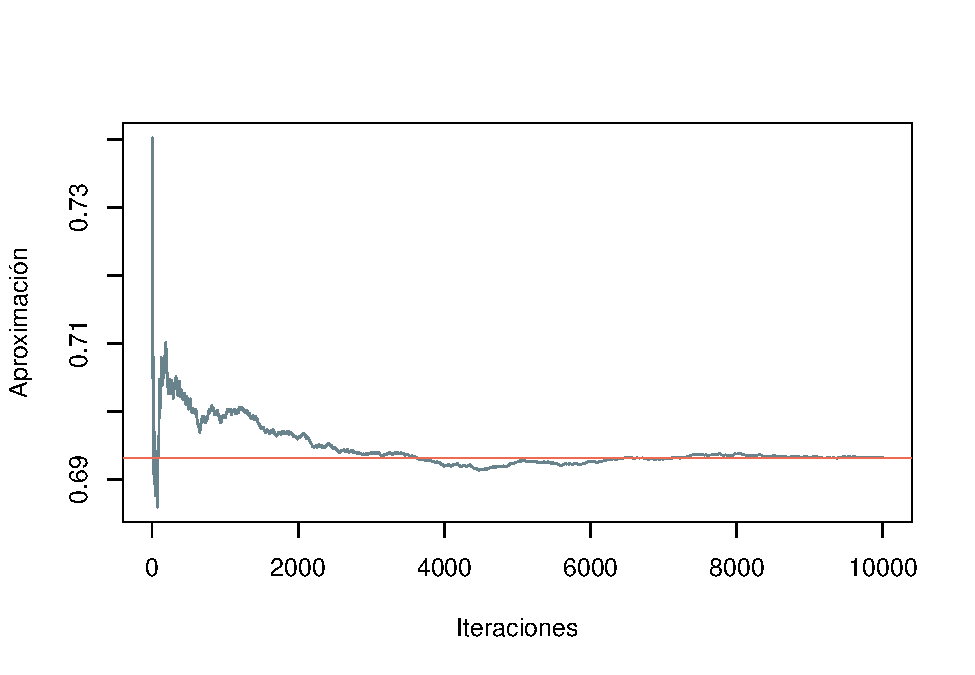
\includegraphics{tarea2_files/figure-latex/unnamed-chunk-1-2.pdf}

\begin{Shaded}
\begin{Highlighting}[]
\NormalTok{P\_est1}\OtherTok{=}\FunctionTok{mean}\NormalTok{(Y)}

\NormalTok{e1 }\OtherTok{\textless{}{-}}\NormalTok{(}\FunctionTok{abs}\NormalTok{(P\_est1}\SpecialCharTok{{-}}\FunctionTok{log}\NormalTok{(}\DecValTok{2}\NormalTok{)))}
\end{Highlighting}
\end{Shaded}

\begin{Shaded}
\begin{Highlighting}[]
\NormalTok{e1}
\end{Highlighting}
\end{Shaded}

\begin{verbatim}
## [1] 4.587881e-05
\end{verbatim}

Concluya que con la función considerada, el algrotimo de integración por
Montecarlo arroja un error absoluto de 4.587881e-05 al estimar ln(2).

\newpage

\hypertarget{ejercicio-2}{%
\section{Ejercicio 2}\label{ejercicio-2}}

\textbf{Usando la metodología de Muestreo por Importancia, si }
\(X \sim N(0.5,0.5)\) \textbf{estime:}

\begin{enumerate}
\def\labelenumi{\alph{enumi}.}
\tightlist
\item
  \(P(X \leq -5)\)
\end{enumerate}

\begin{Shaded}
\begin{Highlighting}[]
\FunctionTok{pnorm}\NormalTok{(}\DecValTok{6}\NormalTok{,}\AttributeTok{mean =} \FloatTok{0.5}\NormalTok{,}\AttributeTok{sd =}\NormalTok{ (}\FloatTok{0.5}\SpecialCharTok{\^{}}\NormalTok{(}\DecValTok{1}\SpecialCharTok{/}\DecValTok{2}\NormalTok{)),}\AttributeTok{lower.tail =}\NormalTok{ F)}
\end{Highlighting}
\end{Shaded}

\begin{verbatim}
## [1] 3.678924e-15
\end{verbatim}

Concluya que la \(P(X \leq -5) = 3.678924e-15\).

\begin{enumerate}
\def\labelenumi{\alph{enumi}.}
\setcounter{enumi}{1}
\tightlist
\item
  Estime el error absoluto de la estimación del punto a:
\end{enumerate}

\begin{Shaded}
\begin{Highlighting}[]
\NormalTok{n }\OtherTok{\textless{}{-}}\DecValTok{10}\SpecialCharTok{\^{}}\DecValTok{4} \CommentTok{\# Tamaño de la muestra}
\NormalTok{A }\OtherTok{\textless{}{-}}\FunctionTok{rexp}\NormalTok{(n) }\SpecialCharTok{+} \DecValTok{6}

\NormalTok{g }\OtherTok{\textless{}{-}}\FunctionTok{Vectorize}\NormalTok{(}\ControlFlowTok{function}\NormalTok{(x) ((}\DecValTok{1}\SpecialCharTok{/}\NormalTok{pi) }\SpecialCharTok{*} \FunctionTok{exp}\NormalTok{(}\SpecialCharTok{{-}}\NormalTok{(x}\FloatTok{{-}0.5}\NormalTok{)}\SpecialCharTok{\^{}}\DecValTok{2}\NormalTok{)}\SpecialCharTok{/}\NormalTok{(}\FunctionTok{exp}\NormalTok{(}\SpecialCharTok{{-}}\NormalTok{x}\SpecialCharTok{+}\DecValTok{6}\NormalTok{))))}

\NormalTok{Y2}\OtherTok{\textless{}{-}}\FunctionTok{g}\NormalTok{(A)}

\NormalTok{M}\OtherTok{\textless{}{-}}\FunctionTok{matrix}\NormalTok{(}\FunctionTok{c}\NormalTok{(}\FunctionTok{mean}\NormalTok{(Y2),}\FunctionTok{pnorm}\NormalTok{(}\DecValTok{6}\NormalTok{,}\AttributeTok{mean =} \FloatTok{0.5}\NormalTok{,}\AttributeTok{sd =}\NormalTok{ (}\FloatTok{0.5}\SpecialCharTok{\^{}}\NormalTok{(}\DecValTok{1}\SpecialCharTok{/}\DecValTok{2}\NormalTok{)), }\AttributeTok{lower.tail =}\NormalTok{ F),}
            \FunctionTok{abs}\NormalTok{(}\FunctionTok{mean}\NormalTok{(Y2)}\SpecialCharTok{{-}}\FunctionTok{pnorm}\NormalTok{(}\DecValTok{6}\NormalTok{,}\AttributeTok{mean =} \FloatTok{0.5}\NormalTok{,}\AttributeTok{sd =}\NormalTok{ (}\FloatTok{0.5}\SpecialCharTok{\^{}}\NormalTok{(}\DecValTok{1}\SpecialCharTok{/}\DecValTok{2}\NormalTok{)), }\AttributeTok{lower.tail =}\NormalTok{ F)),}
            \FunctionTok{sqrt}\NormalTok{(}\FunctionTok{var}\NormalTok{(Y2)}\SpecialCharTok{/}\FunctionTok{sqrt}\NormalTok{(}\DecValTok{10}\SpecialCharTok{\^{}}\DecValTok{4}\NormalTok{))),}\AttributeTok{ncol=}\DecValTok{4}\NormalTok{, }\AttributeTok{byrow=}\ConstantTok{TRUE}\NormalTok{)}

\FunctionTok{colnames}\NormalTok{(M) }\OtherTok{\textless{}{-}} \FunctionTok{c}\NormalTok{(}\StringTok{"Estimacion"}\NormalTok{, }\StringTok{"Valor Real"}\NormalTok{,}\StringTok{"Error Absoluto"}\NormalTok{,}\StringTok{"Error Estandar"}\NormalTok{)}

\NormalTok{M}
\end{Highlighting}
\end{Shaded}

\begin{verbatim}
##        Estimacion   Valor Real Error Absoluto Error Estandar
## [1,] 2.056013e-15 3.678924e-15   1.622911e-15   4.619617e-16
\end{verbatim}

Conculuya que el error absoluto es de 1.622911e-15 al utilizar la
metodología de Muestreo por Importancia.

\end{document}
